% Segment G: Estimation with TMLE in R
% BUILD:
%   Rscript pneumonia_tmle_technical.R
%   pdflatex -interaction=nonstopmode -halt-on-error SegmentG_TMLE.tex
%   pdflatex -interaction=nonstopmode -halt-on-error SegmentG_TMLE.tex
\documentclass[aspectratio=169]{beamer}

\usetheme{metropolis}
\usefonttheme{professionalfonts}
\usepackage[utf8]{inputenc}
\usepackage{amsmath,amssymb,bm}
\usepackage{booktabs}
\usepackage{graphicx}
\usepackage{lmodern}
\usepackage{microtype}
\usepackage{xcolor}
\usepackage{listings}
\usepackage{tikz}
\usetikzlibrary{arrows.meta,calc,positioning}
\pgfdeclarelayer{background}
\pgfsetlayers{background,main}

\definecolor{accent}{HTML}{4A9EFF}
\definecolor{slate}{HTML}{23373B}
\definecolor{danger}{HTML}{C4473A}
\definecolor{support}{HTML}{2F7D6D}

\setbeamercolor{structure}{fg=accent}
\setbeamercolor{background canvas}{bg=white}
\setbeamercolor{alerted text}{fg=danger}
\setbeamercolor{progress bar}{fg=accent,bg=accent}
\setbeamercolor{frametitle}{fg=white,bg=slate}
\setbeamerfont{frametitle}{series=\bfseries}
\metroset{progressbar=frametitle,block=fill}
\setbeamertemplate{navigation symbols}{}
\setbeamertemplate{footline}{}
\setbeamersize{text margin left=0.68cm,text margin right=0.68cm}
\makeatletter
\setlength{\metropolis@progressinheadfoot@linewidth}{1.6pt}
\makeatother

\lstset{
  basicstyle=\ttfamily\scriptsize,
  keywordstyle=\color{accent}\bfseries,
  commentstyle=\color{black!52},
  stringstyle=\color{support},
  showstringspaces=false,
  breaklines=true,
  columns=fullflexible,
  keepspaces=true,
  frame=single,
  rulecolor=\color{black!15},
  backgroundcolor=\color{black!2},
  xleftmargin=5pt,
  xrightmargin=5pt,
  aboveskip=3pt,
  belowskip=3pt
}

\newcommand{\sourcefile}[1]{\texttt{\detokenize{#1}}}
\newcommand{\slidesource}[1]{\note{[Sources]\par #1}}

\title{Estimation with TMLE in R}
\subtitle{From Navigator plan to targeted estimate}
\author{Andy Wilson and Kathryn Morrison}
\institute{Module G}
\date{August 5, 2026 - 4:20--4:55 ET}

\begin{document}

\begin{frame}[plain]
  \begin{tikzpicture}[remember picture,overlay]
    \node[anchor=north east]
      at ([xshift=-0.6cm,yshift=-0.5cm]current page.north east)
      {
\includegraphics[width=2.9cm]{art/InStats_RWL.png}};
    \node[anchor=west,text=slate,
          font=\bfseries\fontsize{25.5}{30}\selectfont]
      at ([xshift=1.4cm,yshift=1.55cm]current page.west)
      {Estimation with TMLE in R};
    \node[anchor=west,text=accent,font=\fontsize{14}{18}\selectfont]
      at ([xshift=1.42cm,yshift=0.72cm]current page.west)
      {From Navigator plan to targeted estimate};
    \draw[black!16,line width=0.5pt]
      ([xshift=1.42cm,yshift=0.05cm]current page.west) --
      ([xshift=8.2cm,yshift=0.05cm]current page.west);
    \node[anchor=west,text=slate,
          font=\bfseries\fontsize{10.5}{13}\selectfont]
      at ([xshift=1.42cm,yshift=-0.62cm]current page.west)
      {Module G \(\cdot\) Estimation};
    \node[anchor=west,text=black!55,font=\fontsize{9.5}{12}\selectfont]
      at ([xshift=1.42cm,yshift=-1.18cm]current page.west)
      {August 5, 2026 \(\cdot\) 4:20--4:55 ET};
    \node[anchor=west,text=black!60,font=\fontsize{9.5}{12}\selectfont]
      at ([xshift=1.42cm,yshift=-2.30cm]current page.west)
      {Andy Wilson \(\cdot\) Kathryn Morrison};
  \end{tikzpicture}
  \slidesource{Visual system adapted from
    \sourcefile{modules/D/SegmentD_Roadmap.tex}.}
\end{frame}

\begin{frame}{The Navigator Carries the Study Plan into Estimation}
  \small
  \begin{columns}[T]
    \begin{column}{0.54\textwidth}
      \textbf{Scientific question}

      \vspace{0.35em}
      In the synthetic pneumonia cohort, what is the effect of baseline
      pneumococcal vaccination on 12-month hospitalization risk?

      \vspace{0.7em}
      \textbf{Target}
      \[
        \Psi = E\!\left[Y^{(1)}\right] - E\!\left[Y^{(0)}\right]
      \]
      A marginal risk difference.
    \end{column}
    \begin{column}{0.42\textwidth}
      \textbf{Observed data}
      \begin{itemize}
        \item \(A\): baseline vaccination
        \item \(Y\): hospitalization by 12 months
        \item \(W\): age, prior pneumonia, prior vaccine
      \end{itemize}

      \vspace{0.4em}
      Estimation holds the population, outcome, adjustment set, and time
      horizon constant.
    \end{column}
  \end{columns}
  \slidesource{Analysis plan from
    \sourcefile{modules/F/causal-roadmap-pneumonia-worked-example.md};
    estimand notation follows Petersen and van der Laan (2014).}
\end{frame}

\begin{frame}{The Pneumonia Example Uses a Defined Cohort and Adjustment Set}
  \small
  \begin{columns}[T]
    \begin{column}{0.38\textwidth}
      \begin{block}{Fixed synthetic cohort}
        \begin{tabular}{@{}lr@{}}
          Participants & 5,000 \\
          Vaccinated & 1,627 \\
          Unvaccinated & 3,373 \\
          Hospitalizations & 334
        \end{tabular}
      \end{block}

      \vspace{0.5em}
      The age distribution is centered near 65. The sufficient adjustment
      set is \(\{\)age, prior pneumonia, prior vaccine\(\}\).
    \end{column}
    \begin{column}{0.58\textwidth}
      \centering
      \resizebox{\linewidth}{!}{%
      \begin{tikzpicture}[
        node distance=0.9cm and 1.25cm,
        v/.style={draw=black!25,rounded corners=2pt,fill=black!2,
                  minimum width=2.2cm,minimum height=0.62cm,align=center},
        a/.style={v,draw=accent,very thick,fill=accent!8},
        outcome/.style={v,draw=support,very thick,fill=support!8}
      ]
        \node[v] (age) {age};
        \node[v,below=of age] (pp) {prior pneumonia};
        \node[v,below=of pp] (pv) {prior vaccine};
        \node[a,right=2.0cm of pp] (A) {\(A\): vaccinated};
        \node[outcome,right=2.1cm of A] (Y) {\(Y\): hospitalization};
        \draw[-{Latex[length=2.2mm]},black!55] (age) -- (pp);
        \draw[-{Latex[length=2.2mm]},black!55]
  (age.west) to[bend right=35] (pv.west);
        \draw[-{Latex[length=2.2mm]},black!55] (age) -- (A);
        \draw[-{Latex[length=2.2mm]},black!55] (pp) -- (A);
        \draw[-{Latex[length=2.2mm]},black!55] (pv) -- (A);
        \draw[-{Latex[length=2.2mm]},black!55] (age.east) to[bend left=24] (Y.north);
        \draw[-{Latex[length=2.2mm]},black!55] (pp.east) to[bend left=8] (Y.west);
        \draw[-{Latex[length=2.2mm]},black!55] (pv.east) to[bend right=24] (Y.south);
        \draw[-{Latex[length=2.4mm]},accent,very thick] (A) -- (Y);
      \end{tikzpicture}%
      }

      \vspace{0.5em}
      The same baseline causes help explain vaccination and pneumonia risk.
    \end{column}
  \end{columns}
  \slidesource{Counts from
    \sourcefile{data/pneumonia_data.csv}; structural equations from
    \sourcefile{simulate_pneumonia_data.R}.}
\end{frame}

\begin{frame}{The Crude Association Reflects Confounding by Indication}
  \small
  \begin{columns}[c]
    \begin{column}{0.31\textwidth}
      \centering
      {\color{accent}\fontsize{28}{32}\selectfont\bfseries 7.19\%}

      vaccinated risk
    \end{column}
    \begin{column}{0.08\textwidth}
      \centering
      {\Large\(-\)}
    \end{column}
    \begin{column}{0.31\textwidth}
      \centering
      {\color{slate}\fontsize{28}{32}\selectfont\bfseries 6.43\%}

      unvaccinated risk
    \end{column}
    \begin{column}{0.25\textwidth}
      \begin{block}{Crude RD}
        \centering
        \(\mathbf{+0.76}\) percentage points
      \end{block}
    \end{column}
  \end{columns}

  \vspace{0.9cm}
  Participants with higher baseline pneumonia risk were more likely to be
  vaccinated. The crude contrast therefore mixes the treatment effect with
  baseline differences between treatment groups.
  \slidesource{Observed risks calculated from
    \sourcefile{data/pneumonia_data.csv}; causal structure from
    \sourcefile{simulate_pneumonia_data.R}.}
\end{frame}

\begin{frame}{Four Estimators Address the Same Risk-Difference Target}
  \small
  \begin{tabular}{@{}p{0.22\textwidth}p{0.29\textwidth}p{0.39\textwidth}@{}}
    \toprule
    \textbf{Estimator} & \textbf{Main model} & \textbf{How it forms the contrast} \\
    \midrule
    Crude & None & Compares the two observed treatment groups \\
    G-computation & \(Q(A,W)=E(Y\mid A,W)\) &
      Predicts outcomes under \(A=1\) and \(A=0\), then averages \\
    IPW & \(g(W)=P(A=1\mid W)\) &
      Reweights observed outcomes to balance measured \(W\) \\
    TMLE & \(Q\) and \(g\) &
      Targets the outcome fit for \(\Psi\), then uses the influence curve \\
    \bottomrule
  \end{tabular}

  \vspace{0.65cm}
  \begin{block}{The comparison is informative because the target stays fixed}
    Only the estimation strategy changes.
  \end{block}
  \slidesource{Estimator definitions follow Hernan and Robins (2020),
    van der Laan and Rose (2011), and the reviewed code in
    \sourcefile{pneumonia_tmle_example.R}.}
\end{frame}

\begin{frame}{G-Computation Standardizes Outcome Predictions}
  \small
  \begin{columns}[T]
    \begin{column}{0.52\textwidth}
      Learn the conditional outcome mean:
      \[
        Q(A,W)=E(Y\mid A,W).
      \]

      For every participant, obtain
      \[
        \widehat Q(1,W_i)
        \quad\text{and}\quad
        \widehat Q(0,W_i).
      \]

      Then standardize over the cohort:
      \[
        \widehat\Psi_{\mathrm{gcomp}}
        =\frac{1}{n}\sum_{i=1}^n
        \left\{\widehat Q(1,W_i)-\widehat Q(0,W_i)\right\}.
      \]
    \end{column}
    \begin{column}{0.43\textwidth}
      \begin{block}{In this example}
        Parametric g-computation:

        \vspace{0.35em}
        \centering
        {\color{accent}\Large\bfseries \(-3.28\) pp}
      \end{block}

      \vspace{0.5em}
      Standardization compares vaccination strategies in the same measured
      covariate distribution.
    \end{column}
  \end{columns}
  \slidesource{Formula and estimate from
    \sourcefile{pneumonia_tmle_example.R}; standardization discussion follows
    Hernan and Robins (2020).}
\end{frame}

\begin{frame}{The Treatment Model Estimates Vaccination Probability}
  \small
  \begin{columns}[T]
    \begin{column}{0.49\textwidth}
      Learn the treatment mechanism:
      \[
        g(W)=P(A=1\mid W).
      \]

      It describes how vaccination varies with measured baseline history.

      \vspace{0.55em}
      IPW uses \(g(W)\) to reweight observed outcomes:
      \[
        \widehat\Psi_{\mathrm{IPW}}=-2.94\text{ pp}.
      \]
    \end{column}
    \begin{column}{0.47\textwidth}
      TMLE also uses \(g(W)\) through the clever covariate:
      \[
        H(A,W)=\frac{A}{g(W)}
          -\frac{1-A}{1-g(W)}.
      \]

      \vspace{0.45em}
      \(H(A,W)\) connects treatment assignment to the residuals from the
      initial outcome model.
    \end{column}
  \end{columns}
  \slidesource{Treatment-model and clever-covariate definitions follow
    van der Laan and Rose (2011); estimate from
    \sourcefile{pneumonia_tmle_example.R}.}
\end{frame}

\begin{frame}{Overlap Informs the Positivity Assessment}
  \begin{columns}[c]
    \begin{column}{0.66\textwidth}
      \centering
      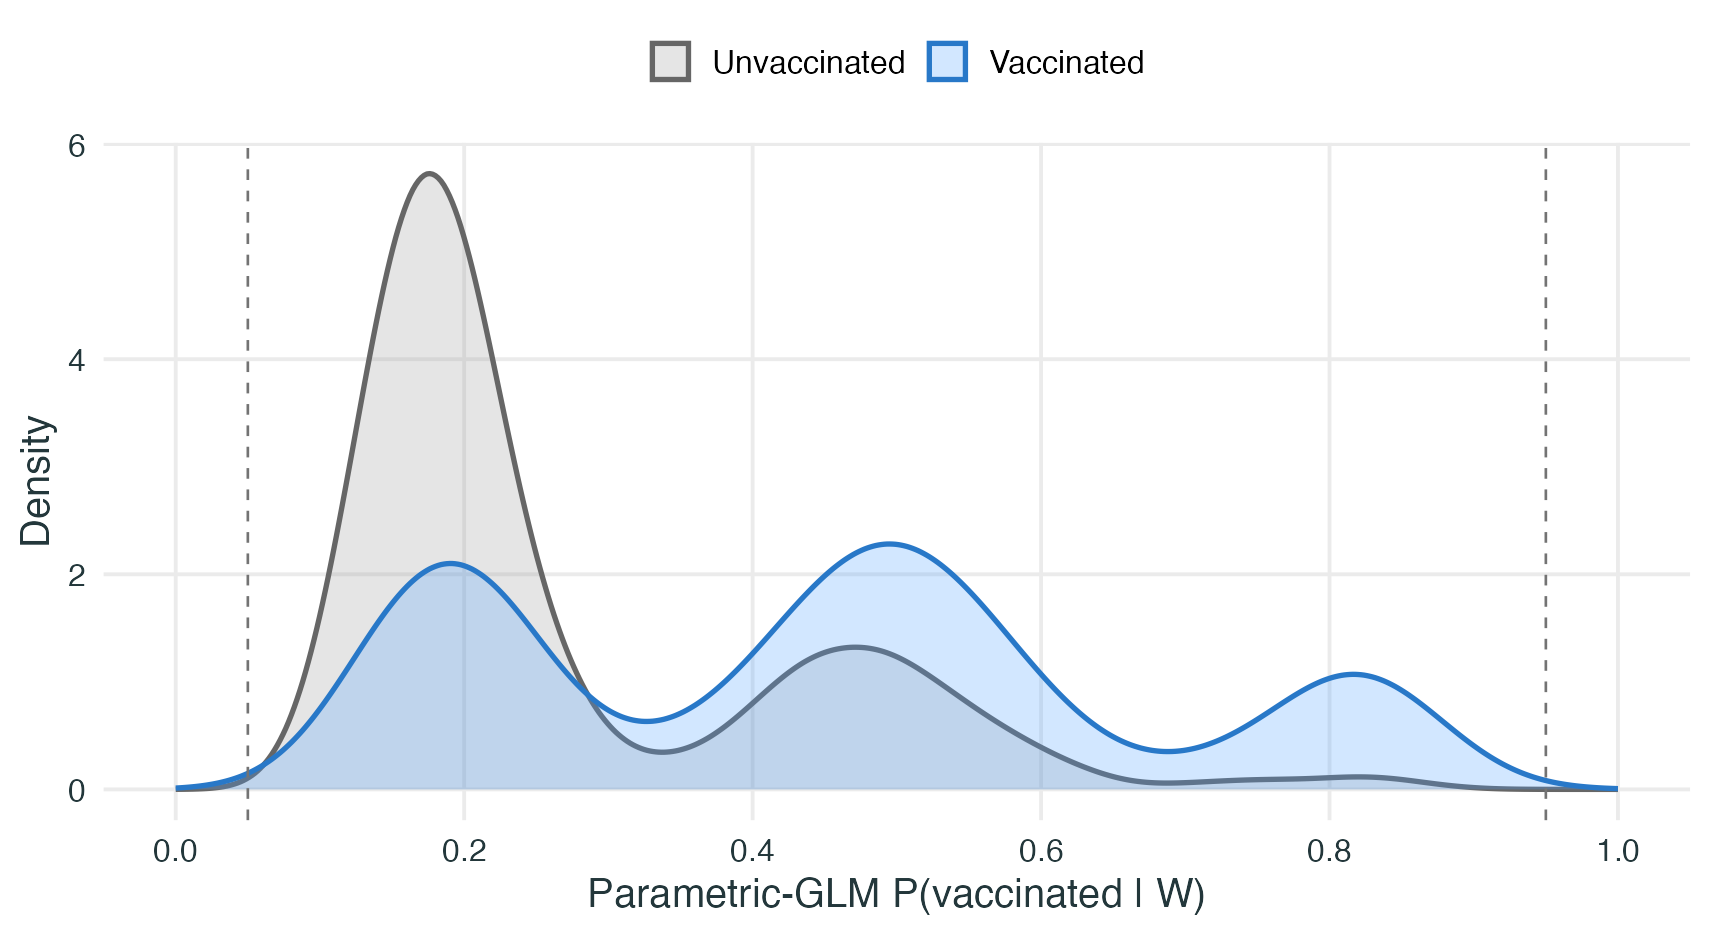
\includegraphics[width=\linewidth]{art/propensity_overlap.png}
    \end{column}
    \begin{column}{0.30\textwidth}
      \small
      \begin{block}{Observed diagnostic}
        Estimated propensity range:
        \[
          0.077\ \text{to}\ 0.909.
        \]
        No fitted values fall outside \([0.05,0.95]\).
      \end{block}

      The treatment groups share support across the measured covariate
      distribution in this synthetic cohort.
    \end{column}
  \end{columns}
  \slidesource{Figure generated by
    \sourcefile{pneumonia_tmle_technical.R}; positivity discussion follows
    Petersen et al. (2012).}
\end{frame}

\begin{frame}{TMLE Combines the Outcome and Treatment Models}
  \small
  \centering
  \begin{tikzpicture}[
    box/.style={draw=black!20,rounded corners=2pt,fill=black!2,
                minimum width=2.45cm,minimum height=1.0cm,align=center},
    key/.style={box,draw=accent,very thick,fill=accent!8}
  ]
    \node[box] (q) {\(\widehat Q(A,W)\)\\outcome fit};
    \node[box,right=1.0cm of q] (g) {\(\widehat g(W)\)\\treatment fit};
    \node[key,right=1.0cm of g] (target) {targeting\\update};
    \node[box,right=1.0cm of target] (psi) {\(\widehat\Psi\) and CI\\risk difference};
    % Route the outcome-fit arrow over the treatment-fit box: both
    % nuisance models feed the targeting step in parallel.
    \draw[-{Latex[length=2.4mm]},thick,black!45] (q.north) -- ++(0,0.48cm) -| (target.north);
    \draw[-{Latex[length=2.4mm]},thick,black!45] (g) -- (target);
    \draw[-{Latex[length=2.4mm]},thick,accent] (target) -- (psi);
  \end{tikzpicture}

  \vspace{0.85cm}
  \begin{columns}[T]
    \begin{column}{0.47\textwidth}
      The targeting step makes a focused update to the initial outcome
      predictions for the chosen risk-difference parameter.
    \end{column}
    \begin{column}{0.47\textwidth}
      Double robustness uses information from both nuisance models; causal
      interpretation still relies on the Navigator's identification
      assumptions.
    \end{column}
  \end{columns}
  \slidesource{TMLE workflow follows van der Laan and Rose (2011) and
    \sourcefile{SegmentG_TMLE_Technical_Supplement.tex}.}
\end{frame}

\begin{frame}[fragile]{A Compact R Implementation Produces the Targeted Estimate}
  \begin{lstlisting}[language=R]
d <- read.csv("data/pneumonia_data.csv")
W <- d[c("age", "priorPneumonia", "priorVaccine")]
A <- d$A
Y <- d$Y

learners <- c("SL.glm", "SL.glmnet", "SL.ranger")
set.seed(2026)
fit <- tmle(
  Y = Y, A = A, W = W,
  Q.SL.library = learners,
  g.SL.library = learners,
  V.Q = 3, V.g = 3
)

fit$estimates$ATE$psi
fit$estimates$ATE$CI
  \end{lstlisting}

  \vspace{0.25em}
  \small
  Full live script: \sourcefile{pneumonia_tmle_example.R}.
  \slidesource{Executable code from
    \sourcefile{pneumonia_tmle_example.R}; package API from tmle 2.1.1.}
\end{frame}

\begin{frame}{Diagnostics and Reproducibility Accompany the Estimate}
  \small
  \begin{columns}[T]
    \begin{column}{0.47\textwidth}
      \textbf{Data and target}
      \begin{itemize}
        \item Fixed 5,000-row synthetic CSV
        \item \(A\), \(Y\), and baseline \(W\) coded explicitly
        \item Marginal 12-month risk difference
      \end{itemize}

      \vspace{0.35em}
      \textbf{Support}
      \begin{itemize}
        \item Propensity range: 0.077 to 0.909
        \item Treatment-specific densities overlap
      \end{itemize}
    \end{column}
    \begin{column}{0.47\textwidth}
      \textbf{Nuisance learning}
      \begin{itemize}
        \item GLM, penalized GLM, and random forest
        \item Three-fold cross-validation for workshop runtime
      \end{itemize}

      \vspace{0.35em}
      \textbf{Audit trail}
      \begin{itemize}
        \item Standalone generator and value check
        \item Saved results, diagnostics, figures, and session info
      \end{itemize}
    \end{column}
  \end{columns}
  \slidesource{Diagnostics and outputs from
    \sourcefile{pneumonia_tmle_technical.R} and
    \sourcefile{simulate_pneumonia_data.R}.}
\end{frame}

\begin{frame}{Adjustment Changes the Estimated Direction and Magnitude}
  \centering
  \vspace{-0.2cm}
  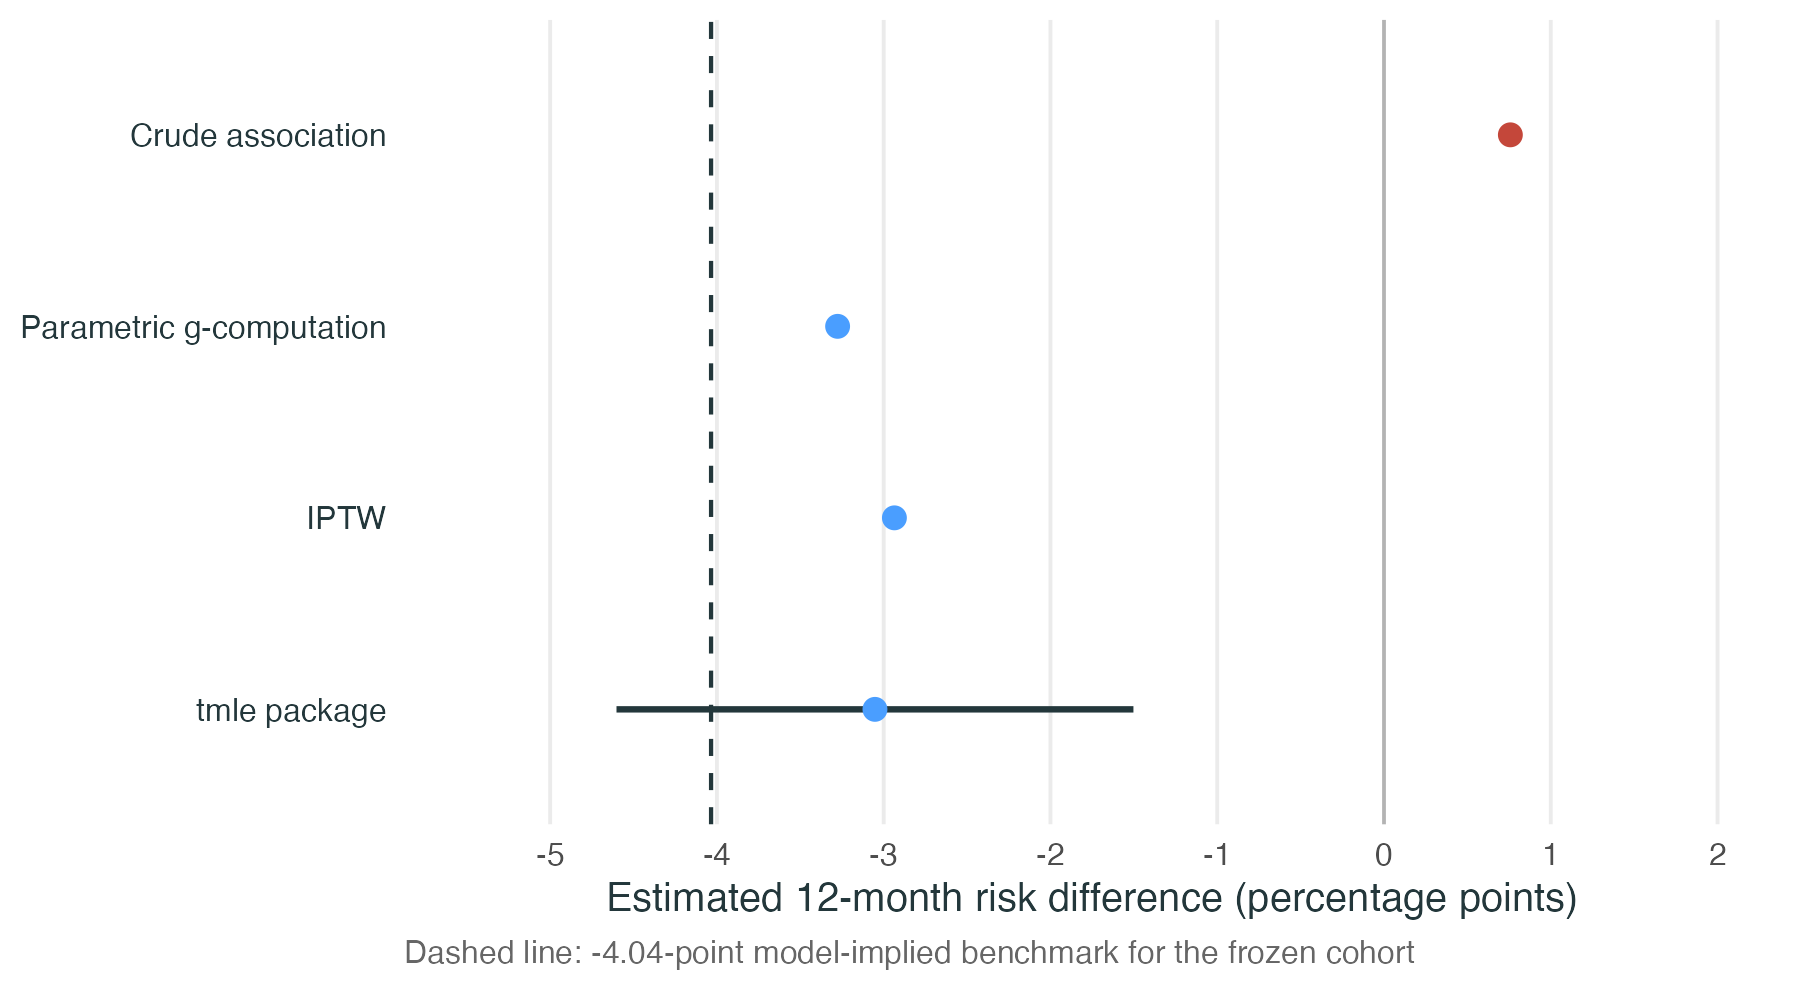
\includegraphics[width=0.82\textwidth]{art/estimator_comparison.png}

  \vspace{-0.1cm}
  \footnotesize
  The adjusted estimators are similar in this synthetic example. That
  agreement supports an implementation check; it does not assess unmeasured
  confounding.
  \slidesource{Figure generated by
    \sourcefile{pneumonia_tmle_technical.R}; benchmark generated by
    \sourcefile{simulate_pneumonia_data.R}.}
\end{frame}

\begin{frame}{The TMLE Estimate Is a 3.05-Percentage-Point Risk Reduction}
  \small
  \begin{columns}[c]
    \begin{column}{0.45\textwidth}
      \centering
      {\color{accent}\fontsize{30}{35}\selectfont\bfseries \(-3.05\) pp}

      \vspace{0.35em}
      \(\text{95\% CI: }-4.60\text{ to }-1.50\text{ pp}\)
    \end{column}
    \begin{column}{0.50\textwidth}
      \begin{block}{Interpretation}
        If the stated assumptions identify the target, vaccination is
        estimated to reduce 12-month pneumonia hospitalization risk by about
        3.05 events per 100 people in this synthetic cohort.
      \end{block}

      \vspace{0.45em}
      The model-implied benchmark for the frozen cohort is \(-4.04\) percentage points.
      It is available here only because the teaching data generator is known.
    \end{column}
  \end{columns}

  \vspace{0.7cm}
  \centering
  \color{black!58}\footnotesize Synthetic teaching result - not clinical evidence.
  \slidesource{Estimate from
    \sourcefile{pneumonia_tmle_example.R}; model-implied benchmark from
    \sourcefile{simulate_pneumonia_data.R}.}
\end{frame}

\begin{frame}{TMLE Inherits the Study's Causal Assumptions}
  \small
  \begin{columns}[T]
    \begin{column}{0.47\textwidth}
      \textbf{Identification}
      \begin{itemize}
        \item Conditional exchangeability given measured \(W\)
        \item Positivity in the target population
        \item Consistency of the treatment and outcome definitions
      \end{itemize}
    \end{column}
    \begin{column}{0.47\textwidth}
      \textbf{Study implementation}
      \begin{itemize}
        \item Accurate treatment and outcome measurement
        \item A common time zero and 12-month follow-up
        \item Appropriate handling of missingness and selection
      \end{itemize}
    \end{column}
  \end{columns}

  \vspace{0.7cm}
  \begin{block}{Scope}
    These assumptions belong to the study and causal model. TMLE carries them
    into an estimator with flexible nuisance fitting and influence-curve
    uncertainty.
  \end{block}
  \slidesource{Assumptions follow Hernan and Robins (2020), Petersen and
    van der Laan (2014), and the Navigator roadmap.}
\end{frame}

\begin{frame}{The Estimate Goes Back Into the Roadmap}
  \small
  \centering
  \begin{tikzpicture}[
    stage/.style={draw=black!18,rounded corners=2pt,minimum width=2.05cm,
                  minimum height=1.15cm,align=center,fill=black!2},
    final/.style={stage,draw=accent,very thick,fill=accent!8}
  ]
    \node[stage] (q) {\textbf{Question}\\population, \(A\), \(Y\)};
    \node[stage,right=0.42cm of q] (m) {\textbf{Causal model}\\DAG and time zero};
    \node[stage,right=0.42cm of m] (i) {\textbf{Identification}\\assumptions};
    \node[stage,right=0.42cm of i] (e) {\textbf{Estimand}\\risk difference};
    \node[final,right=0.42cm of e] (a) {\textbf{Estimate}\\TMLE and CI};
    \begin{pgfonlayer}{background}
      \draw[-{Latex[length=2.3mm]},thick,black!45] (q) -- (m);
      \draw[-{Latex[length=2.3mm]},thick,black!45] (m) -- (i);
      \draw[-{Latex[length=2.3mm]},thick,black!45] (i) -- (e);
      \draw[-{Latex[length=2.3mm]},thick,accent] (e) -- (a);
    \end{pgfonlayer}
  \end{tikzpicture}

  \vspace{1.0cm}
  \begin{block}{One continuous analysis}
    The same study plan now connects the scientific question to a reproducible
    estimate, uncertainty interval, and assumption-calibrated interpretation.
  \end{block}

  \vspace{0.45cm}
  \textbf{Next resource:} the technical supplement opens the \(Q\), \(g\),
  targeting, and influence-curve steps.
  \slidesource{Roadmap adapted from
    \sourcefile{modules/D/SegmentD_Roadmap.tex}; technical details in
    \sourcefile{SegmentG_TMLE_Technical_Supplement.tex}.}
\end{frame}

\end{document}
